\documentclass[xcolor=dvipsnames]{beamer} 
\usepackage[croatian]{babel}
\usepackage[utf8]{inputenc}
\usepackage{graphicx}
\usecolortheme[named=Blue]{structure} 
\usetheme[height=7mm]{Boadilla} 
\setbeamertemplate{items}[ball] 
\setbeamertemplate{blocks}[rounded][shadow=true] 

\title[]{Ekspertni sustavi}
\author[V. Berger]{Viktor Berger}
\institute[UMBC]{
  Fakultet elektrotehnike i računarstva\\
}
\date[March 15]{15. Ožujak, 2014}

\begin{document}


\begin{frame}[plain]
  \titlepage
\end{frame}



\begin{frame}{Povijest}


\begin{itemize}
	\item pokušaji stvaranja inteligentnih strojeva kroz povijest
  	\item 50-ih i 60-ih pokušaji razvoja sofisticiranih tehnika zaključivanja
  	\item cilj razvoj univerzalnog sustava zaključivanja - neuspjeh
  	\item drugi pristup  sustavi temeljeni na znanju
\end{itemize}


\end{frame}






\begin{frame}{Znanje}
Kako je najlakše izraziti ljudsko znanje?
\begin{itemize}
	\item Većinu ljudskog znanja moguće je prikazati \textbf{AKO-ONDA} pravilima
  	\item \textbf{AKO} je temperatura pacijenta veća od 38 stupnjeva \textbf{ONDA} treba prepisati lijek za snižavanje temperature
  	\item \textbf{AKO} je svjetlo na semaforu crveno \textbf{ONDA} se zaustavi
  	\item Takva se pravila nazivaju \textbf{produkcijska pravila}
\end{itemize}
\end{frame}



\begin{frame}{Znanje}

Važan korak u rješavanju problema umjetnom inteligencijom: \newline
Redukcija područja problema
\begin{figure}
\center

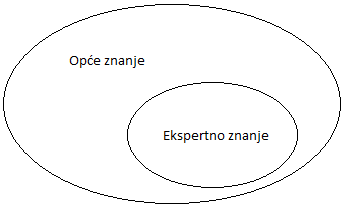
\includegraphics[scale=0.5]{img/znanje.png}

\end{figure}

\textbf{Ekspertno znanje} (područno znanje) je specifično znanje 
koje se odnosi na određeno usko područje, domenu 
(medicinu, financije, pravo itd.), za razliku od općeg znanja 
rješavanja problema

\end{frame}



\begin{frame}{Ekspertni sustav}

\begin{itemize}
	\item \textbf{Ekspertni sustavi} čine granu umjetne inteligencije koja koristi 
	specijalizirano(ekspertno) znanje iz neke problemske domene da bi 
	riješila problem na razini ljudskog eksperta
	\item \textbf{Osnovna shema sustava temeljenog na znanju -ekspertnog sustava}
\end{itemize}

\begin{figure}
\center

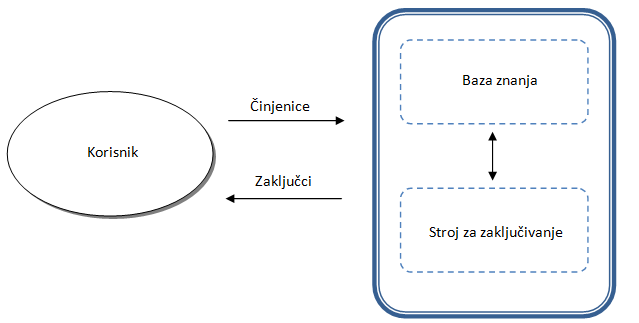
\includegraphics[scale=0.5]{img/shema.png}

\end{figure}
\end{frame}




\begin{frame}{Inspiracija}

\begin{itemize}
	\item Model ljudskog spoznajnog procesa se oponaša u ekspertnom sustavu
	\item Osjeti stimuliraju mozak podražajima. Takvi podražaju aktiviraju znanje u našoj \textbf{dugotrajnoj memorij}i (u prod. sustavu to su ako – onda pravila)
	\item  \textbf{Kratkotrajna memorija} – privremena pohrana znanja za vrijeme postupka zaključivanja – predstavlja broj «granula znanja» koje mogu biti simultano razmatrane - (pravila koja mogu biti istodobno aktivirana) 
	\item \textbf{Spoznajni proces} - pronalazi pravila koja će biti aktivirana podražajima – (u prod. sustavu odgovara mu stroj za zaključivanje, on pronalazi pravila, rješava konflikte) 
\end{itemize}
\end{frame}



\begin{frame}{Izgradnja sustava}
Pokušaj formaliziranja ekspertnog znanja računalom $\rightarrow$ ekspertni sustav
\begin{figure}
\center

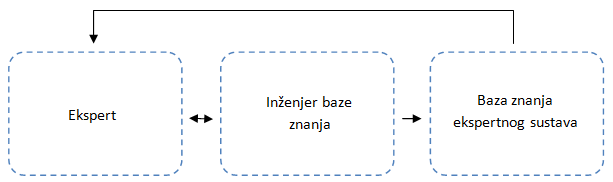
\includegraphics[scale=0.5]{img/konstr.png}

\end{figure}

Prednosti:
\begin{itemize}
\item izgrađeni na temelju znanja više eksperata - repozitorij ekspertnog znanja za neko područje
\item mogu se umnožiti i biti u širokoj uporabi
\end{itemize}

\end{frame}


\begin{frame}{Produkcijska pravila}

\begin{figure}
\center

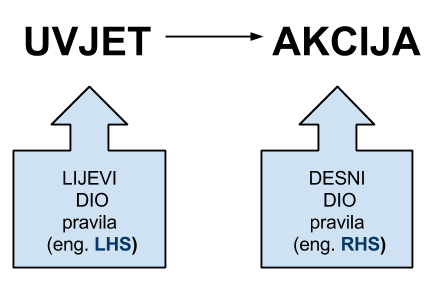
\includegraphics[scale=0.5]{img/HS.png}

\end{figure}

\end{frame}

\begin{frame}{Definicija sustava}
\textbf{EKSPERTNI SUSTAV} definiran je sa:
\begin{itemize}
	\item \textbf{ SKUPOM PRODUKCIJSKIH PRAVILA}(produkcija je par uvjet-akcija)
	\item \textbf{RADNOM MEMORIJOM} (baza činjenica koja sadrži opis tekućeg stanja svijetau postupku zaključivanja)
	\item \textbf{CIKLUSOM PODUDARANJE-DJELOVANJE} To je upravljački mahanizam koji se sastoji od slijeda akcija: podudaranje uzoraka  – izbor pravila rješavanjem konflikata - izvršavanje pravila 
\end{itemize}

 U užem smislu baza znanja) $\rightarrow$ skup produkcijskih pravila. 
Baza znanja kaže se i baza pravila.
\end{frame}



\begin{frame}{Načini zaključivanja}
Postoje dva glavna načina napredovanja prema 
zaključcima:
\begin{itemize}
\item \textbf{ULANČAVANJE PRAVILA PREMA NAPRIJED} -započinjanje sa znanim podacima i napredovanje prema zaključku
\item \textbf{ULANČAVANJE PRAVILA UNATRAG} - izbor mogućeg zaključka (hipoteza) i pokušaj dokazivanja valjanosti hipoteze traženjem valjanih  potpora
\end{itemize}
\end{frame}


\begin{frame}{Načini zaključivanja}

\begin{itemize}
\item \textbf{Ulančavanje prema naprijed} - kada ima malo podataka i puno mogućih rješenja(za problemske domene koje uključuju sintezu: za dizajniranje, planiranje, raspoređivanje, za nadzor i dijagnostiku sustava za rad u stvarnim vremenu)
\end{itemize}


\begin{figure}
\center
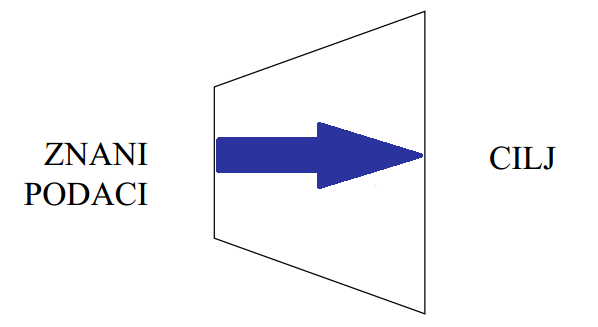
\includegraphics[scale=0.5]{img/naprijed.png}
\end{figure}

\end{frame}

\begin{frame}{Načini zaključivanja}

\begin{itemize}
\item \textbf{Ulančavanje unatrag} razuman je izbor kada je malo mogućih zaključaka/ciljeva i puno znanih podataka. (Za probleme dijagnosticiranja, klasificiranja)
\end{itemize}


\begin{figure}
\center
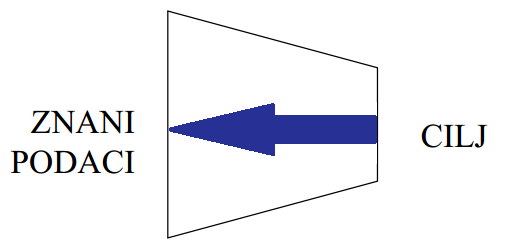
\includegraphics[scale=0.5]{img/natrag.png}
\end{figure}


\begin{itemize}
\item Izbor metode zaključivanja ovisi o osobinama problemske domene i o načinu zaključivanja eksperta
\end{itemize}

\end{frame}

\begin{frame}{Ulančavanje prema naprijed}

\textbf{STROJ ZA ZAKLJUČIVANJE} je upravljački mahanizam koji u postupku ulančavanja prema naprijed izvodi sljedeće korake:
\begin{itemize}
\item \textbf{Podudaranje} - upravljački ciklus započinje podudaranjem stanja u radnoj memoriji s LIJEVIM dijelom produkcijskog pravila
\item \textbf{Razrješavanje konflikata} – ako je tijekom podudaranja nađeno više pravila koja su omogućena – izabire se pravilo najvećeg prioriteta
\item \textbf{Izvršavanje (paljenje) pravila} – izvršavanje desnog dijela (akcija) produkcijskog pravila rezultira:
\begin{itemize}
\item novom činjenicom koja je dodana u radnu memoriju (novo tekuće stanje svijeta, ili engl. current state of the world), ili
\item novim pravilom koje je dodano u bazu znanja i može biti razmatrano za izvršavanje u sljedećim ciklusima
\end{itemize}
\end{itemize}
\end{frame}


\begin{frame}{Ulančavanje prema naprijed}

\begin{itemize}
\item Oblikuj stog inicijalno sastavljen od najvažnijih ciljeva (hipoteza) koje treba dokazati
\item Na vrhu stoga je hipoteza koju treba dokazati. Ako je stog prazan, onda je KRAJ
\item Izdvoji sva pravila koja mogu zadovoljavati dani cilj (tj. izdvoji sva pravila čija se DESNA strana podudara s ciljem)

\end{itemize}

\end{frame}










\end{document}


